\documentclass{article}

\usepackage{fancyhdr} % Required for custom headers
\usepackage{lastpage} % Required to determine the last page for the footer
\usepackage{extramarks} % Required for headers and footers
\usepackage[usenames,dvipsnames]{color} % Required for custom colors
\usepackage{graphicx} % Required to insert images
\usepackage{listings} % Required for insertion of code
\usepackage{courier} % Required for the courier font
\usepackage{lipsum} % Used for inserting dummy 'Lorem ipsum' text into the template
\usepackage{hyperref}
\usepackage{multirow}
\usepackage{tabularx}
\usepackage{longtable}
\usepackage{listings}
\usepackage{subfigure}
\usepackage{afterpage}
\usepackage{amsmath,amssymb}            
\usepackage{rotating}  
\usepackage{fancyhdr}
\usepackage{graphicx}
\usepackage{amsthm}
\usepackage[scriptsize]{caption} 
\hyphenation{a-gen-tiz-za-zio-ne}
% Margins
\topmargin=-0.45in
\evensidemargin=0in
\oddsidemargin=0in
\textwidth=6.5in
\textheight=9.0in
\headsep=0.25in

\linespread{1.1} % Line spacing

% Set up the header and footer
\pagestyle{fancy}
\lhead{\hmwkAuthorName} % Top left header
\chead{\hmwkClass\ (\hmwkClassInstructor\ \hmwkClassTime): \hmwkTitle} % Top center head
\rhead{\firstxmark} % Top right header
\lfoot{\lastxmark} % Bottom left footer
\cfoot{} % Bottom center footer
\rfoot{Page\ \thepage\ of\ \protect\pageref{LastPage}} % Bottom right footer
\renewcommand\headrulewidth{0.4pt} % Size of the header rule
\renewcommand\footrulewidth{0.4pt} % Size of the footer rule

\setlength\parindent{0pt} % Removes all indentation from paragraphs

\usepackage{listings}
\usepackage{color}

\definecolor{dkgreen}{rgb}{0,0.6,0}
\definecolor{gray}{rgb}{0.5,0.5,0.5}
\definecolor{mauve}{rgb}{0.58,0,0.82}

\lstset{frame=tb,
  language=Java,
  aboveskip=3mm,
  belowskip=3mm,
  showstringspaces=false,
  columns=flexible,
  basicstyle={\small\ttfamily},
  numbers=none,
  numberstyle=\tiny\color{gray},
  keywordstyle=\color{blue},
  commentstyle=\color{dkgreen},
  stringstyle=\color{mauve},
  breaklines=true,
  breakatwhitespace=true
  tabsize=3
}

%----------------------------------------------------------------------------------------
%	DOCUMENT STRUCTURE COMMANDS
%	Skip this unless you know what you're doing
%----------------------------------------------------------------------------------------

% Header and footer for when a page split occurs within a problem environment
\newcommand{\enterProblemHeader}[1]{
\nobreak\extramarks{#1}{#1 continued on next page\ldots}\nobreak
\nobreak\extramarks{#1 (continued)}{#1 continued on next page\ldots}\nobreak
}

% Header and footer for when a page split occurs between problem environments
\newcommand{\exitProblemHeader}[1]{
\nobreak\extramarks{#1 (continued)}{#1 continued on next page\ldots}\nobreak
\nobreak\extramarks{#1}{}\nobreak
}




%----------------------------------------------------------------------------------------
%	NAME AND CLASS SECTION
%----------------------------------------------------------------------------------------

\newcommand{\hmwkTitle}{Design Pattern} % Assignment title
\newcommand{\hmwkDueDate}{Martedi,\ Aprile 15,\ 2014} % Due date
\newcommand{\hmwkClass}{Ingegneria del Software 1} % Course/class
\newcommand{\hmwkClassTime}{} % Class/lecture time
\newcommand{\hmwkClassInstructor}{} % Teacher/lecturer
\newcommand{\hmwkAuthorName}{} % Your name

%----------------------------------------------------------------------------------------
%	TITLE PAGE
%----------------------------------------------------------------------------------------

\title{
\vspace{2in}
\textmd{\textbf{\hmwkClass:\ \hmwkTitle}}\\
\normalsize\vspace{0.1in}\small{Due\ on\ \hmwkDueDate}\\
\vspace{0.1in}\large{\textit{\hmwkClassInstructor\ \hmwkClassTime}}
\vspace{3in}
}

\author{\textbf{\hmwkAuthorName}}
\date{} % Insert date here if you want it to appear below your name

%----------------------------------------------------------------------------------------

\begin{document}

\maketitle

%----------------------------------------------------------------------------------------
%	TABLE OF CONTENTS
%----------------------------------------------------------------------------------------

%\setcounter{tocdepth}{1} % Uncomment this line if you don't want subsections listed in the ToC

\newpage
\tableofcontents
\newpage



%----------------------------------------------------------------------------------------
\section{Introduction}


\section{Structural Patterns Theory}
Structural patterns are used when classes and objects are \emph{composed to form larger structures}.

\subsection{Adapter}
\label{Adapter}
\subsubsection{Goal}
Makes one interface \emph{the adaptee's} conform to another, providing a uniform abstraction of different interfaces. 

\subsubsection{Structure}
%\begin{figure}[h!]
%  \centering
%    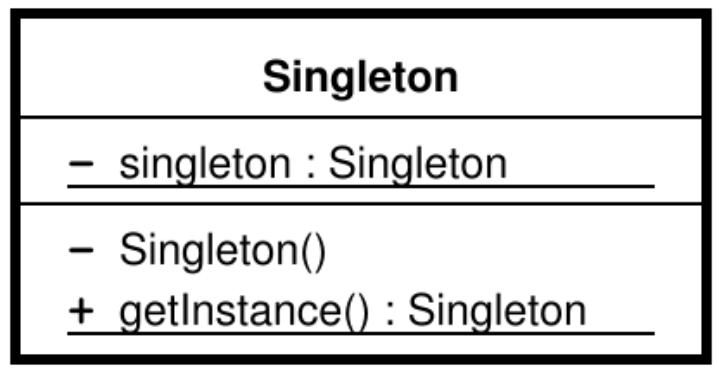
\includegraphics[width=0.3\textwidth]{Img/SingletonUML.png}
%     \caption{Singleton UML}
%     \label{SingletonUML}
%\end{figure}
General idea: make the class ensuring that \textbf{only} one instance is creating. The idea is to make the class able to intersect creation of new objects and to provide an easy way to access the instance.

\subsubsection{Implementation}
The class which must be singleton (in this case named as $Singleton$) has
\begin{itemize}
\item a \textbf{static} attribute $singleton$ of type $Singleton$
\item a \textbf{private} constructor (in this case $Singleton()$) which could have also parameters
\item a \textbf{public} and \textbf{static} method $getInstance()$ which returns the instance of the singleton class. The method $getInstance$ is the only way to instantiate the object and thus can guarantee the access of the unique copy referenced by the $static$ attribute singleton. 
\end{itemize}


\subsubsection{Examples}
\textbf{Printer spooler}\\
 Although there can be many printers in a system, there should be only one printer spooler.
 
 \textbf{File system, Window manager}\\
 There should be only one file system and one window manager.
 
\subsubsection{When to use it}
\begin{itemize}
\item when it is necessary to instantiate  a class exactly once (the class must be accessible to the client from a well known access point).
\item when it is necessary to control the access to the instance (it is possible to control $who$ and $when$ can access the instance).
\item it can reduce the number of instances of an object in the system
\item allows the refinement of the class and provides a way to configure the application to get the instance of the class you need at run-time
\item it allows using a similar approach to control the number of instances of a class at run-time
\end{itemize}

\subsubsection{Additional references}
For additional information the interested reader may refer to \url{http://www.javaworld.com/article/2073352/core-java/simply-singleton.html} and to~\cite{gamma1994design}.


\subsection{Factory Method (Virtual Constructor)}
\subsubsection{Goal}
Define an interface for creating an object, but let free the sub-classes decide which class to instantiate.

\subsubsection{Structure}

%\begin{figure}[h!]
%  \centering
%    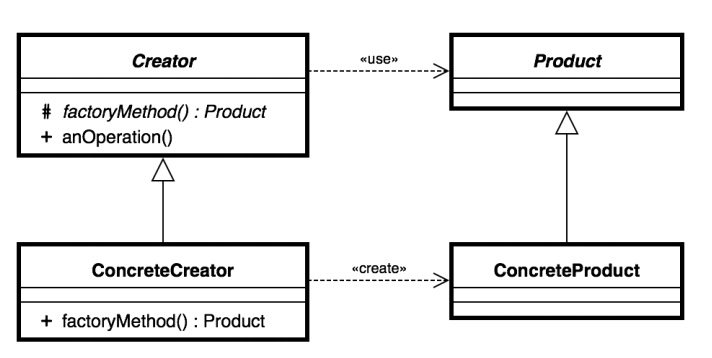
\includegraphics[width=0.8\textwidth]{Img/FactoryMethod.png}
%     \caption{Factory Method UML.}
%     \label{FactoryMethod}
%\end{figure}

\begin{itemize}
\item the creation of the object is hidden inside a specific method called factory: \emph{a method which returns an object but is not the constructor of that object}
\item the factory method decides the strategy to be employed in the allocation of the object
\end{itemize}


Components involved:

\begin{itemize}
\item  \textbf{Product} defines the interface of the products that the factory method creates.
\item \textbf{Concrete Product} are the concrete product the factory creates
\item  \textbf{Creator} 
\begin{itemize}
\item declares the factory method, which returns the Product
\item it is also possible to provide a default implementation of the factory method 
\end{itemize}
\item \textbf{Concrete Creator} overrides the factory method of the abstract creator to return a specific Concrete Product
\end{itemize}

\subsubsection{Implementation}
To describe the implementation we refer to figure~\ref{FactoryMethod}. Other implementations and designs may be provided.
\begin{itemize}
\item the \textbf{Creator} is an abstract class with an abstract public or protected factory method. If a default implementation is provided the method is not abstract. It uses the Abstract class Product
\item  \textbf{ConcreteCreator} overrides the factory method of the Creator, in this case it also forces the method to be public. The Factory Method of the ConcreteCreator returns the ConcreteProduct. It uses the ConcreteProduct class.
\item  \textbf{Product} is an AbstractClass which describes the Product
\item \textbf{ConcreteProduct} is a concrete class which extends the AbstractClass Product
\end{itemize}

\subsubsection{Examples}
Let's consider a drawing application. We may have two classes one for drawing the application interface (DrawingApplication) and one for driving the document (DrawingDocument). The Application class is responsible for creating these Drawing elements when the user requires them, for example when he clicks on the Open or New menus.

\subsubsection{When to use it}
\begin{itemize}
\item it is not possible to anticipate a priori the class to be created
\item the designer wants to delegate the responsibility to create the class to one of several helper subclasses, and you want to localize the knowledge of the class to create in the subclasses.
\end{itemize}
%----------------------------

\subsubsection{Additional references}
A different implementation of the Factory Method Pattern can be found in~\cite{gamma1994design}.


\subsection{Abstract Factory (Kit)}
\subsubsection{Goal}
The goal is to create an interface which allows to create families of \textbf{related or dependent objects}, \textit{without specifying} their concrete classes. 

\subsubsection{Structure}

%\begin{figure}[h!]
%  \centering
%    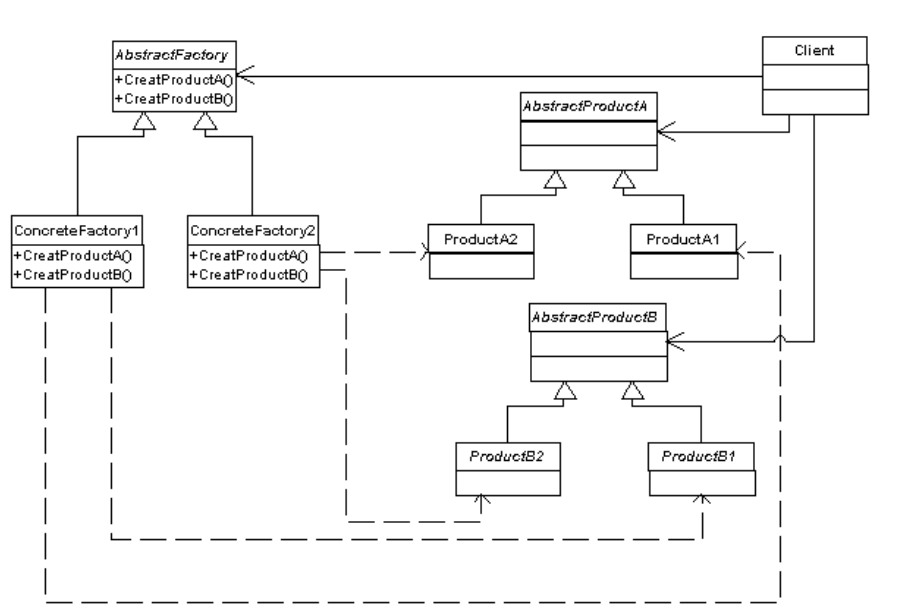
\includegraphics[width=0.8\textwidth]{Img/AbstractFactoryUML.png}
%     \caption{Abstract Factory UML.}
%     \label{AbstractFactoryUML}
%\end{figure}

Using this pattern an abstract framework (factory) is defined, which allows to create objects that follow a general pattern. At run-time the abstract factory is paired with any concrete factory that allows to create the objects that follow the concrete pattern. In other words, the Abstract Factory is a super-factory which creates other factories (Factory of factories). The UML of Figure~\ref{AbstractFactoryUML} is composed by the following classes:
\begin{itemize}
\item \emph{AbstractFactory}: is an abstract class (see the italic style of the text), which declares the interface for the operations that allows to create \emph{abstract} products
\item \emph{ConcreteFactory}: are the concrete classes that allows to create \emph{concrete} products (Note the hierarchical relation between the AbstractFactory and the ConcreteFactory). Each product is a family of related dependent objects AbstractProductA and AbstractProductB, and in particular, for the ConcreteFactory1 the products are ProductA1 and ProductB1, while for the ConcreteFactory2 the products are ProductA2 and ProductB2 (Note the uses relation between the Factories and the products).
\item \emph{AbstractProduct}:  declares an abstract product which can be aggregated to other products using appropriate factories
\item \emph{ConcreteProduct}: are  concrete products which extends  particular abstract products.
\item \emph{Client}: instantiate a specific ConcreteFactory (depending on its necessities) to obtain specific products.
\end{itemize}

Note: usually only a single instance of a ConcreteFactory class is created at run-time. The AbstractFactory defers the creation of products to the ConcreteFactories.

\subsubsection{Implementation}
\begin{itemize}
\item \emph{AbstractFactory} only declare the interface for the creating the products
\item \emph{ConcreteFactory} are \emph{singleton}. A \emph{factory method} is defined for each product. 
\end{itemize}


\subsubsection{Examples}
\emph{Window Interface}\\
Consider a user interface that must support multiple devices, such as laptops, cellphones. Different interfaces must be creating depending on the device which runs the application (e.g., different type of scroll bars, windows, buttons). To be portable, the application should not be hard-coded to a particular look and feel. The instantiation and the designing new look-and-feels must be easy. The example is inspired by~\cite{gamma1994design}.



\subsubsection{Pro and Cons}
\begin{itemize}
\item it requires a concrete factory subclass for each product even if the families differ only slightly
\item if many families are possible think about using a \emph{prototype pattern} inside the factory (You can store classes inside a concrete factory that create the various concrete products in variables, much like prototypes).
\item AbstractFactory usually define a \emph{different operation} for each kind of product it is possible to create, i.e., for each product there is a signature in the AbstractFactory Interface. This implies that \emph{to add a new product} you must add the \emph{signature in the abstract factory} and all the sub Factory-classes. A \textbf{more flexible} but \textbf{less safe} design is to add a parameter in the operations to create objects. This parameter specifies the object to be created (e.g., an enum).
\item All the products are returned to the client as abstract interfaces to the product. The client is not able to make safe assumption on the type of the product.
\end{itemize}








\section{Creational Patterns Exercises}
\subsection{Singleton}

\subsubsection{EagerSingleton}
\begin{lstlisting}
package creationalpatterns.singleton;

/**
 * 
 * @author claudio menghi
 * The singleton class ensures that only a unique instance of the class can be ever created
 * Note that 
 * -	the object is created and instantiated before its first use
 * -	if the object is big and it is not used a lot of memory is occupied and not used
 * -	it is thread safe
 */
public class EagerSingleton {

	/**
	 * contains the unique instance of the {@link EagerSingleton} class
	 * if the object is big it can occupy a lot of memory if not used
	 */
	private static EagerSingleton uniqueInstance=new EagerSingleton();
	
	/**
	 * The constructor of the {@link EagerSingleton} class is hided (either private or protected). 
	 * If protected it is possible to call the constructor from the subclasses 
	 */
	private EagerSingleton(){
		
	}
	
	/**
	 * returns the pointer to the unique instance of the class
	 * @return the pointer to the unique instance of the {@link EagerSingleton} class
	 */
	public static EagerSingleton getInstance(){
		return uniqueInstance;
	}
}
\end{lstlisting}

\subsubsection{Use of EagerSingleton}
\begin{lstlisting}
package creationalpatterns.singleton;

/**
 * this class shows an example of use of the EagerSingleton pattern
 * @author claudio menghi
 *
 */
public class EagerSingletonMain {

	public static void main(String[] args) {
		
		// declares a new instance of EagerSingleton 
		EagerSingleton eagerSing1;
		// declares a new instance of EagerSingleton 
		EagerSingleton eagerSing2;
		
		// gets an instance of an EagerSingleton
		eagerSing1=EagerSingleton.getInstance();
		
		// gets another (the same) instance of an EagerSingleton
		eagerSing2=EagerSingleton.getInstance();
		
		/*
		 *  compare the references of the two objects using ==  
		 */
		if(eagerSing1==eagerSing2){
			System.out.println("The two references are equals: they point to the same object");
		}
		else{
			System.out.println("The two references are different");
		}
	}
}
\end{lstlisting}

\subsubsection{LazySingleton}

\begin{lstlisting}
package creationalpatterns.singleton;

/**
 * @author Claudio Menghi
 * The singleton class ensures that only a unique instance of the class can be ever created
 * Note that 
 * -	the object is instantiated only when needed
 * -	it does not occupy additional memory as the {@link EagerSingleton}
 * -	it is NOT THREAD safe -> it does not work for multithreads applications
 */
public class LazySingleton {
	
	/**
	 * contains the unique instance of the {@link LazySingleton} class
	 */
	private static LazySingleton uniqueInstance;
	// other attributes
	
	/**
	 * The constructor of the {@link LazySingleton} class is hided (either private or protected). 
	 * If protected it is possible to call the constructor from the subclasses 
	 */
	private LazySingleton(){
		// initialization of other attributes
	}
	
	/**
	 * returns the pointer to the unique instance of the class
	 * @return the pointer to the unique instance of the {@link LazySingleton} class
	 */
	public static LazySingleton getInstance(){
		
		// if the instance has not already been created,  the new instance is created
		if(uniqueInstance==null){
			uniqueInstance=new LazySingleton();
		}
		// the instance is returned
		return uniqueInstance;
	}	
}
\end{lstlisting}

\subsubsection{Use of LazySingleton}
\begin{lstlisting}
package creationalpatterns.singleton;

public class LazySingletonMain {

	public static void main(String[] args) {
		
		// declares a new instance of LazySingleton 
		LazySingleton lazySing1;
		// declares a new instance of LazySingleton 
		LazySingleton lazySing2;
		
		// gets an instance of an LazySingleton
		lazySing1=LazySingleton.getInstance();
		
		// gets another (the same) instance of an LazySingleton
		lazySing2=LazySingleton.getInstance();
		
		/*
		 *  compare the references of the two objects using ==  
		 */
		if(lazySing1==lazySing2){
			System.out.println("The two references are equals: they point to the same object");
		}
		else{
			System.out.println("The two references are different");
		}
	}
}
\end{lstlisting}

\subsubsection{Synchronization problems in the use of LazySingleton}
\begin{lstlisting}
package creationalpatterns.singleton;

public class LazySingletonSynchronization {
   private static LazySingleton singleton = null;
	
   public static void main(String[] args) throws InterruptedException {
		
	   // Both threads call Singleton.getInstance().
      Thread threadOne = new Thread(new SingletonRunnable());
      Thread threadTwo = new Thread(new SingletonRunnable());
      threadOne.start();
      threadTwo.start();
      threadOne.join();
      threadTwo.join();
   }
   private static class SingletonRunnable implements Runnable {
      public void run() {
    	 /*
    	  * add 
    	  * try {
				Thread.currentThread().sleep(1000);
			} catch (InterruptedException e) {
				// TODO Auto-generated catch block
				e.printStackTrace();
			}
			in the constructor of the LazySingleton 
    	  */
         // Get a reference to the singleton.
         LazySingleton s = LazySingleton.getInstance();
         // Protect singleton member variable from
         // multithreaded access.
         synchronized(LazySingleton.class) {
            if(singleton == null) // If local reference is null...
               singleton = s;     // ...set it to the singleton
         }
         // Local reference must be equal to the one and
         // only instance of Singleton; otherwise, we have two
                  // Singleton instances.
         if(s==singleton){
        	 System.out.printf("The local reference is equal to singleton\n");
         }
         else{
        	 System.out.printf("The local reference is not equal to the singleton\n");
         }
      }
   }
}
\end{lstlisting}



\subsubsection{Synchronized Lazy Singleton}
\begin{lstlisting}
/**
 * @author Claudio Menghi
 * The {@link SynchronizedLazySingleton} alters the {@link LazySingleton} 
 * to guarantee the correct behavior of the {@link LazySingleton} in case of multithreading 
 */
public class SynchronizedLazySingleton {
	/**
	 * contains the unique instance of the {@link SynchronizedLazySingleton} class
	 */
	private static SynchronizedLazySingleton uniqueInstance;
	
	private SynchronizedLazySingleton(){
		// costruttore
	}
	
	/**
	 * returns the pointer to the unique instance of the class. The syncronized attribute guarantees the correct behaviour
	 * is a multithreading environment
	 * @return the pointer to the unique instance of the {@link SynchronizedLazySingleton} class
	 */
	public static synchronized SynchronizedLazySingleton getInstance(){
		// metodi synchronized possono essere inefficienti
		if (uniqueInstance == null){
			uniqueInstance = new SynchronizedLazySingleton();
		}
		return uniqueInstance;
			
	}
}
\end{lstlisting}

\subsubsection{Use of the Synchronized Lazy Singleton}
\begin{lstlisting}
package creationalpatterns.singleton;


public class SynchronizedLasySingletonMain {
	private static SynchronizedLazySingleton singleton = null;
	
	   public static void main(String[] args) throws InterruptedException {
			
		   // Both threads call Singleton.getInstance().
	      Thread threadOne = new Thread(new SingletonRunnable());
	      Thread threadTwo = new Thread(new SingletonRunnable());
	      threadOne.start();
	      threadTwo.start();
	      threadOne.join();
	      threadTwo.join();
	   }
	   private static class SingletonRunnable implements Runnable {
	      public void run() {
	    	 /*
	    	  * add 
	    	  * try {
					Thread.currentThread().sleep(1000);
				} catch (InterruptedException e) {
					// TODO Auto-generated catch block
					e.printStackTrace();
				}
				in the constructor of the LazySingleton 
	    	  */
	         // Get a reference to the singleton.
	    	  SynchronizedLazySingleton s = SynchronizedLazySingleton.getInstance();
	         // Protect singleton member variable from
	         // multithreaded access.
	         synchronized(SynchronizedLazySingleton.class) {
	            if(singleton == null) // If local reference is null...
	               singleton = s;     // ...set it to the singleton
	         }
	         // Local reference must be equal to the one and
	         // only instance of Singleton; otherwise, we have two
	                  // Singleton instances.
	         if(s==singleton){
	        	 System.out.printf("The local reference is equal to singleton\n");
	         }
	         else{
	        	 System.out.printf("The local reference is not equal to the singleton\n");
	         }
	      }
	   }
}
\end{lstlisting}


\subsubsection{Enum Singleton}

\begin{lstlisting}
package creationalpatterns.singleton;

/**
 * Metodo alternativo e thread safe. Non supporta ereditarieta'
 * @author claudio menghi
 */
public enum EnumSingleton {
	INSTANCE;
	public static EnumSingleton getInstance(){
		return INSTANCE;
	}
}
\end{lstlisting}


\subsection{Factory Method}

\subsubsection{Product}

\begin{lstlisting}
/**
 * 
 */
package creationalpatterns.factorymethod;

import java.util.ArrayList;
import java.util.List;

/**
 * @author claudio menghi
 * contains the abstract product
 */
public abstract class Pizza {
	/**
	 * contains the name of the {@link Pizza}
	 */
	private String name;
	/**
	 * contains the sauce used to make the {@link Pizza}
	 */
	private String sauce;
	/**
	 * contains the List of the ingredients of the {@link Pizza}
	 */
	private List<String> ingredients;
	
	/**
	 * creates a new {@link Pizza}
	 * @param name is the name of the {@link Pizza}
	 * @param sauce is the sauce used to make the {@link Pizza}
	 */
	protected Pizza(String name, String sauce){
		this.name=name;
		this.sauce=sauce;
		this.ingredients=new ArrayList<String>();
	}

	/**
	 * add the ingredient ingredient to the {@link Pizza}
	 * @param ingredient is the ingredient to be added to the pizza
	 */
	public void addIngredient(String ingredient){
		if(ingredient==null){
			throw new NullPointerException("The ingredient to be added cannot be null");
		}
		this.ingredients.add(ingredient);
		
	}
	
	public void prepare() {
		System.out.println("Preparazione di Pizza " + name);
		System.out.println("Aggiungi la salsa " + sauce);
		System.out.println("Aggiungi gli ingredienti:" );
		for (String ingrediente: ingredients){
			System.out.println(ingrediente);
		}		
	}
	public void cook(){
		System.out.println("Cotta in forno per 10 minuti");
	}
	public void cut(){
		System.out.println("Taglia la pizza a fette");
	}
	
	public String getNome(){
		return name;
	}
}
\end{lstlisting}


\begin{lstlisting}
package creationalpatterns.factorymethod;

/**
 * contains a specific type of {@link Pizza} and in particular {@link PizzaGenovese}
 * @author Claudio1
 */
public class PizzaGenovese extends Pizza {

	/**
	 * creates a new {@link PizzaGenovese}
	 */
	public PizzaGenovese() {
		super("Al pesto", "Pesto DOC");
		this.addIngredient("Pomodorini");
		this.addIngredient("Grana a scaglie");
	}
}
\end{lstlisting}

\begin{lstlisting}
package creationalpatterns.factorymethod;

/**
 * contains a specific type of {@link Pizza} and in particular {@link PizzaNapoletana}
 * @author Claudio1
 */
public class PizzaNapoletana extends Pizza {

	/**
	 * creates a new {@link PizzaNapoletana}
	 */
	public PizzaNapoletana(){
		super("Margherita", "Spesso e soffice");
		this.addIngredient("Mozzarella di Bufala");
		this.addIngredient("Basilico Fresco");
	}
}
\end{lstlisting}

\begin{lstlisting}
package creationalpatterns.factorymethod;

/**
 * contains a specific type of {@link Pizza} and in particular {@link PizzaTaggiasca}
 * @author Claudio1
 */
public class PizzaTaggiasca extends Pizza {

	/**
	 * creates a new {@link PizzaTaggiasca}
	 */
	public PizzaTaggiasca(){
		super("Pizza alle Olive", "Sottile e croccante");
		this.addIngredient("Pomodorini");
		this.addIngredient("Olive taggiasche");
	}
}
\end{lstlisting}

\subsubsection{Creator}

\begin{lstlisting}
/**
 * 
 */
package creationalpatterns.factorymethod;

/**
 * is the creator:  an abstract class with an abstract public or protected factory method. 
 * If a default implementation is provided the method is not abstract. It uses the Abstract class Product
 * @author Claudio1
 *
 */
public abstract class Pizzeria {

	/**
	 * is a public method which allows to create the pizza
	 * @param type is the type of the pizza which is ordered
	 * @return the ordered pizza
	 */
	public Pizza orderPizza(String type){
		Pizza pizza;
		pizza = createPizza(type);
		pizza.prepare();
		pizza.cook();
		pizza.cut();
		return pizza;
	}
	/**
	 * is the factory method
	 * @param type is the type of the pizza require
	 * @return the pizza required
	 * @throws IllegalArgumentException if the specific type of pizza is not available
	 */
	protected abstract Pizza createPizza(String type);
}
\end{lstlisting}

\begin{lstlisting}
package creationalpatterns.factorymethod;

/**
 * is a concrete Creator.
 * It overrides the factory method of the Creator. 
 * The Factory Method of the ConcreteCreator returns the ConcreteProduct (the concrete pizza). 
 * It uses the ConcreteProduct class {@link PizzaNapoletana} 
 * @author Claudio1
 *
 */
public class PizzeriaBellaNapoli extends Pizzeria {

	@Override
	public Pizza createPizza(String type) {
		if(!type.equals("margherita")){
			throw new IllegalArgumentException("The pizza "+type+" is not available in the PizzeriaBellaNapoli");
		}
		return new PizzaNapoletana();
	}
}
\end{lstlisting}

\begin{lstlisting}
package creationalpatterns.factorymethod;

/**
 * is a concrete Creator.
 * It overrides the factory method of the Creator. 
 * The Factory Method of the ConcreteCreator returns the ConcreteProduct (the concrete pizza). 
 * It uses the ConcreteProduct class {@link PizzaGenoveses} 
 * @author Claudio1
 *
 */
public class PizzeriaCinqueTerre extends Pizzeria {

	@Override
	protected Pizza createPizza(String type) {
		switch(type){
			case "pesto":
				return new PizzaGenovese();
			case "olive":
				return new PizzaTaggiasca();
			default: 
				throw new IllegalArgumentException("The pizza "+type+" is not available in the PizzeriaCinqueTerre");
		}
	}
}
\end{lstlisting}


\subsubsection{Use of the pattern}
\begin{lstlisting}
package creationalpatterns.factorymethod;

public class Main {

	public static void main(String[] args) {
		Pizzeria bellaNapoli = new PizzeriaBellaNapoli();
		Pizzeria cinqueTerre = new PizzeriaCinqueTerre();
		
		Pizza pizza = bellaNapoli.orderPizza("margherita");
		System.out.println("Valerio ha ordinato la pizza " + pizza.getNome());
		System.out.println("###############");
		
		pizza = cinqueTerre.orderPizza("pesto");
		System.out.println("Carlo ha ordinato la pizza " + pizza.getNome());
	}
}
\end{lstlisting}




\subsection{Abstract Factory}

\subsubsection{Product 1: Sauce}
\begin{lstlisting}
/**
 * 
 */
package creationalpatterns.abstractfactory.sauce;

/**
 * @author Claudio1
 * contains the abstract description of a sauce
 */
public abstract class Sauce {

	/**
	 * @return the String description of the sauce
	 */
	public abstract String toString();
}
\end{lstlisting}

\begin{lstlisting}
/**
 * 
 */
package creationalpatterns.abstractfactory.sauce;

/**
 * @author Claudio1
 * contains a pesto sauce
 */
public class PestoSauce extends Sauce {

	@Override
	public String toString() {
		
		return "Pesto sauce";
	}

}
\end{lstlisting}

\begin{lstlisting}
/**
 * 
 */
package creationalpatterns.abstractfactory.sauce;

/**
 * @author Claudio1
 * contains a Tomato sauce
 */
public class TomatoSauce extends Sauce {

	@Override
	public String toString() {
		return "Tomato sauce";
	}

}

\end{lstlisting}

\subsubsection{Product 2: Ground}
\begin{lstlisting}
/**
 * 
 */
package creationalpatterns.abstractfactory.ground;

/**
 * @author Claudio1
 * contains the abstract description of the ground of the pizza
 */
public abstract class Ground {
	
	/**
	 * @return a {@link String} which describes the ground
	 */
	public abstract String toString();
}
\end{lstlisting}

\begin{lstlisting}
/**
 * 
 */
package creationalpatterns.abstractfactory.ground;

/**
 * @author Claudio1
 *	contains a crisp grpund
 */
public class CrispGround extends Ground {

	@Override
	public String toString() {
		return "Crisp ground";
	}

}
\end{lstlisting}

\begin{lstlisting}
/**
 * 
 */
package creationalpatterns.abstractfactory.ground;

/**
 * @author Claudio1
 * contains a soft gound
 */
public class SoftGround extends Ground {

	@Override
	public String toString() {
		return "Soft ground";
	}

}
\end{lstlisting}

\subsubsection{Factories}
\begin{lstlisting}
/**
 * 
 */
package creationalpatterns.abstractfactory.pizzafactories;

import creationalpatterns.abstractfactory.ground.Ground;
import creationalpatterns.abstractfactory.sauce.Sauce;

/**
 * @author Claudio1
 * is a factory which returns the ingredients of a particular pizza
 */
public abstract class PizzaIngredientFactory {
	/**
	 * returns the {@link Ground} of the pizza
	 * @return the {@link Ground} of the pizza
	 */
	public abstract Ground createGroud();
	/**
	 * returns the {@link Sauce} to be added in the pizza
	 * @return the {@link Sauce} to be added in the pizza
	 */
	public abstract Sauce createSauce();
}
\end{lstlisting}

\begin{lstlisting}
/**
 * 
 */
package creationalpatterns.abstractfactory.pizzafactories;

import creationalpatterns.abstractfactory.ground.Ground;
import creationalpatterns.abstractfactory.ground.SoftGround;
import creationalpatterns.abstractfactory.sauce.Sauce;
import creationalpatterns.abstractfactory.sauce.TomatoSauce;
import creationalpatterns.factorymethod.Pizza;

/**
 * @author Claudio1
 * contains the Factory of a Napoli {@link Pizza}
 */
public class NapoliPizzaIngredientFactory extends PizzaIngredientFactory {

	/**
	 * returns the Ground created in a Genova Pizza Factory which is a {@link SoftGround}
	 * @return a {@link SoftGround}
	 */
	
	@Override
	public Ground createGroud() {
		return new SoftGround();
	}
	/**
	 * returns the {@link Sauce} created in a Genova {@link PizzaIngredientFactory} factory which is a {@link TomatoSauce}
	 * @return a {@link TomatoSauce}
	 */
	
	@Override
	public Sauce createSauce() {
		return new TomatoSauce();
	}

}
\end{lstlisting}

\begin{lstlisting}
/**
 * 
 */
package creationalpatterns.abstractfactory.pizzafactories;

import creationalpatterns.abstractfactory.ground.CrispGround;
import creationalpatterns.abstractfactory.ground.Ground;
import creationalpatterns.abstractfactory.sauce.PestoSauce;
import creationalpatterns.abstractfactory.sauce.Sauce;

/**
 * @author Claudio1
 * contains
 */
public class GenovaPizzaIngredientFactory extends PizzaIngredientFactory {

	/**
	 * returns the Ground created in a Genova Pizza Factory which is a {@link CrispGround}
	 * @return a {@link CrispGround}
	 */
	@Override
	public Ground createGroud() {
		Ground ground = new CrispGround();
		return ground;
		
	}
	/**
	 * returns the {@link Sauce} created in a Genova {@link PizzaIngredientFactory} factory which is a {@link PestoSauce}
	 * @return a {@link PestoSauce}
	 */
	@Override
	public Sauce createSauce() {
		PestoSauce sauce=new PestoSauce();
		return sauce;
	}

}
\end{lstlisting}

\subsubsection{Client}
\begin{lstlisting}
/**
 * 
 */
package creationalpatterns.abstractfactory.pizza;

import creationalpatterns.abstractfactory.ground.Ground;
import creationalpatterns.abstractfactory.pizzafactories.PizzaIngredientFactory;
import creationalpatterns.abstractfactory.sauce.Sauce;

/**
 * @author Claudio1
 * contains the abstract of a Pizza represents a client which is using the {@link PizzaIngredientFactory}
 * 
 */
public class Pizza {
	/**
	 * contains the ground of the {@link Pizza}
	 */
	private Ground ground;
	/**
	 * contains the {@link Sauce} of the {@link Pizza}
	 */
	private Sauce sauce;
	
	/**
	 * creates a new {@link Pizza} with the specified {@link Ground} and {@link Sauce}
	 * @param ground is the {@link Ground} of the {@link Pizza}
	 * @param sauce is the {@link Sauce} of the {@link Pizza}
	 */
	private Pizza(Ground ground, Sauce sauce){
		this.ground=ground;
		this.sauce=sauce;
	}
	
	/**
	 * creates a new {@link Pizza} with the specified {@link PizzaIngredientFactory}
	 * @param factory is the factory which is used to create the {@link Pizza}
	 */
	public Pizza(PizzaIngredientFactory factory){
		this(factory.createGroud(), factory.createSauce());
	}
	/**
	 * returns the {@link String} representation of the {@link Pizza}
	 */
	public String toString(){
		return "ground: "+this.ground.toString()+" \t sauce: "+this.sauce.toString();
	}
}
\end{lstlisting}

\subsubsection{Use of the Factory}

\begin{lstlisting}
/**
 * 
 */
package creationalpatterns.abstractfactory;

import creationalpatterns.abstractfactory.pizza.Pizza;
import creationalpatterns.abstractfactory.pizzafactories.GenovaPizzaIngredientFactory;
import creationalpatterns.abstractfactory.pizzafactories.NapoliPizzaIngredientFactory;

/**
 * @author Claudio1
 *
 */
public class Main {

	/**
	 * @param args
	 */
	public static void main(String[] args) {
		// creates a new GenovaIngridient factory
		GenovaPizzaIngredientFactory genovaFactory=new GenovaPizzaIngredientFactory();
		// creates a new pizza using the ingredients provided by the Genova factory
		Pizza pizzaGenovese=new Pizza(genovaFactory);
		System.out.println(pizzaGenovese);
		
		// creates a new NapoliPizzaIngridient factory
		NapoliPizzaIngredientFactory napoliFactory=new NapoliPizzaIngredientFactory();
		// creates a new pizza using the ingredients provided by a Napoli pizzeria
		Pizza pizzaNapoletana=new Pizza(napoliFactory);
		System.out.println(pizzaNapoletana);
	}
}
\end{lstlisting}


\clearpage
% ---- Bibliography ----




\addcontentsline{toc}{chapter}{Bibliography}
\bibliographystyle{alpha}
\bibliography{StructuralPatterns}
\nocite{*}


\end{document}

